% 
%
% (c) 2025 Autor, ETH Zürich
%
% !TEX root = linalg_I-II_summary.tex
% !TEX encoding = UTF-8
%

\section{Linear Maps}

\begin{definition}{Linear Map}{lin_map}
	Let $V,W$ be vector spaces over $K$. A map $T:V \to W$ is called linear map if:
	\begin{enumerate}
		\item $\forall v_1,v_2 \in V: \; T(v_1 + v_2) =T(v_1) + T(v_2)$
		\item $\forall \alpha \in K, \forall v \in V: \; T(\alpha \cdot v) = \alpha \cdot T(v)$
	\end{enumerate}
	This means that $T:V \to W$ is a map that respects the structures of vector spaces on $(V, +, \cdot), (W, +, \cdot)$.
	We denote the set of all linear maps $T:V \to W$ by $\operatorname{Hom}(V, W)$. Sometimes $\hom_K(V,W)$.
\end{definition}

\begin{proposition}{Properties of Linear Maps}{prop_lin_map}
	Let $V, W$ be vector spaces over a field $K$, and let $T:V \to W$ be a linear map. Then:
	\begin{enumerate}
		\item $\forall n \in \mathbb{N}, a_1, \hdots , a_n \in K, v_1, \hdots , v_n \in V$ we have
		\[
		T\big(\sum_{i=1}^{n} a_i v_i\big) = \sum_{i=1}^{n} a_i T(v_i).
		\]
		\item $T(0_V) = 0_W$.
	\end{enumerate}
	
\end{proposition}

\begin{theorem}{A unique Linear Map}{unique_lin_map}
	Let $V$ be a finite dimensional vector space and $v_1, \hdots ,v_n \in V$ a basis for $V$. Let $w_1, \hdots , w_n \in W$ be arbitrary vectors. Then there exists a unique linear map $T:V \to W$ s.t.
	\[
	T(v_i) = w_i \qquad \forall 1 \leq i \leq n.
	\]
\end{theorem}

\begin{lemma}{Matrix Representation of the Unique Linear Map}{mat_unique_lin_map}
	For every linear transformation $T:K^n \to K^m$ there exists a unique matrix $A \in M_{m\times n}(K)$ s.t. $T = T_A$.
\end{lemma}









\subsection{Kernel \& Image}

\begin{definition}{Kernal and Image}{ker_im}
	Let $V, W$ we vector spaces over $K$ and $T: V \to W$ a linear map.
	\begin{enumerate}
		\item The set 
		\[
		\ker(T) := \{v \in V \;|\; Tv = 0\} \subseteq V
		\]
		is a linear subspace of $V$. It is called the \textbf{kernel of T}.
		\item  The set
		\[
		\operatorname{Im}(T) := \{Tv \;|\; v \in V\} \subseteq W
		\]
		is a linear subspace of $W$. It is called the \textbf{image of T}.
	\end{enumerate}
	With the notation from set theory, we have
	\[
	\ker(T) = T^{-1}(\{0\}), \qquad \operatorname{Im}(T) = T(V).
	\]
\end{definition}

\begin{proposition}{Equivalences for Injective and Surjective}{equiv_inj_surj}
	Let $T:V \to W$ be a linear map. Then:
	\begin{enumerate}
		\item $T$ is injective $\quad \Longleftrightarrow \quad \ker(T) = \{0\}$.
		\item $T$ is surjective $\quad \Longleftrightarrow \quad \operatorname{Im}(T) = W$.
	\end{enumerate}
\end{proposition}

\subsubsection{About Linear Maps}

\begin{definition}{Isomorphism}{iso}
	A linear map $T: V \to W$ is called an \textbf{isomorphism} if there exists a linear map $S:W \to V$ s.t. $S \circ T = \operatorname{id}_{V}$, $T \circ S = \operatorname{id}_{W}$. We say that $V$ is isomorphic to $W$ if there exists an isomorphism $T: V \to W$. We write $V \cong W$.
\end{definition}

\begin{lemma}{Linearity of the Inverse Map}{lin_inv_map}
	Let $T:V \to W$ be a linear map which is bijective. Then the inverse map $T^{1}:W \to V$ is linear. In other words, a linear bijective map is an isomorphism.
\end{lemma}

\begin{lemma}{Composition of Linear Maps}{comp_lin_map}
	Let $T:V \to W$ and $S:W \to U$ be linear maps. Then the composition $S \circ T:V \to U$ is also linear.
\end{lemma}

\begin{definition}{Endomorphism / Automorphism}{endo_auto}
	
	A linear map $T:V \to V$ is sometimes called an \textbf{endomorphism} of $V$. We denote the set of all endomorphisms of $V$ by $\operatorname{End}(V)$. (So, $\operatorname{End}(V) = \operatorname{Hom}(V, V)$.)
	
	A linear map $T:V \to V$ which is an isomorphism is also called an \textbf{automorphism} of $V$.
\end{definition}

\begin{lemma}{Span of a Basis}{span_basis}
	Let $T:V \to W$ be a linear map. Let $v_1, \hdots , v_n$ be a basis of $V$. Then $\operatorname{Im}(T) = \operatorname{Sp}(Tv_1, \hdots , Tv_n)$
\end{lemma}

\begin{theorem}{\textcolor{red}{Rank Theorem}}{rank_thm}
	Let $V, W$ be vector spaces, where $V$ is finite dimensional and let $T: V \to W$ be a linear map. Then
	\[
	\dim \ker(T) + \dim \operatorname{Im}(T) = \dim V.
	\]
\end{theorem}

\begin{proof}
	Define $n := \dim V$. Let $u_1, \hdots , u_k$ be a basis for $\ker(T)$. Note that $\ker(T)$ is finite dimensional, b.c. it is a subspace of $V$, which is finite dimensional. Extend $u_1, \hdots , u_k$ to a basis $u_1, \hdots , u_k, v_1, \hdots , v_{n-k}$ of $V$, which we can do by a previous result. By Lemma \ref{lem*span_basis}, we have that
	\[
	\operatorname{Im}(T) = \operatorname{Sp}(\underbrace{Tu_1, \hdots Tu_2}_{\displaystyle = 0}, Tv_1, \hdots , Tv_{n-k}) = \operatorname{Sp}(Tv_1, \hdots , Tv_{n-k}).
	\]
	We'll show now that $Tv_1, \hdots , Tv_{n-k}$ is linearly independent. To see this, assume that
	\[
	\sum_{i = 1}^{n-k} a_iTv_i = 0,
	\]
	for some $a_1, \hdots a_{n-k} \in K$. Since $T$ is linear we can write this linear combination as
	\[
	T\big(\sum_{i = 1}^{n-k} a_i v_i\big) = 0 \qquad \Longrightarrow \qquad \sum_{i = 1}^{n-k} a_i v_i \in \ker(T).
	\]
	Now, $u_1, \hdots , u_k$ form a basis for $\ker(T)$. So, $\exists \,b_1, \hdots , b_k \in K$ s.t. 
	\begin{align*}
		\sum_{i = 1}^{n-k} a_iv_i &= b_1u_1 + \hdots + b_k u_k\\
		\Longrightarrow \quad b_1u_1 + \hdots + b_ku_k &+ (-a_1)v_1 + \hdots + (-a_{n-k})v_{n-k} = 0.
	\end{align*}
	Since, $u_1, \hdots , u_k, v_1, \hdots , v_{n-k}$ form a basis for $V$, we have that $b_1 = \hdots = b_k = a_1 = \hdots = a_{n-k} = 0$. This shows that $Tv_1, \hdots , Tv_{n-k}$ are linearly independent. Therefore, $Tv_1, \hdots , Tv_{n-k}$ form a basis for $\operatorname{Im}(T)$. Thus,
	\begin{align*}
		\dim \operatorname{Im}(T) &= n - k = \dim V - \dim \ker(T)\\
		\Longrightarrow \quad \dim \ker(T) + \dim \operatorname{Im}(T) &= \dim V. 
	\end{align*}
	\qedhere
\end{proof}

\begin{corollary}{Consequences of the Rank Theorem}{consq_rank_thm}
	Let $T:V \to W$ be a linear map, where $V, W$ are finite dimensional vector spaces. Then the following holds:
	\begin{enumerate}
		\item If $\dim W < \dim V$ then $T$ is \textbf{not} injective.
		\item If $\dim W > \dim V$ then $T$ is \textbf{not} surjective.
		\item If $\dim W = \dim V$ then $T$ is bijective $\Longleftrightarrow$ $T$ is surjective $\Longleftrightarrow$ $T$ is injective.
	\end{enumerate}
\end{corollary}

\begin{corollary}{Equivalence for an Isomorphism}{equiv_iso}
	Two finite dimensional vector spaces $V, W$ are isomorphic if and only if $\dim V = \dim W$.
\end{corollary}

\begin{theorem}{Image of a Set}{im_set}
	Let $T:V \to W$ be an isomorphism between two vector spaces $V, W$.
	Let $S$ be a family of vector in $V$. Write $T(S) := \{Tv\}_{v \in S}$. Then:
	\begin{enumerate}
		\item $S$ is linearly independent if and only if $T(S)$ is linearly independent.
		\item $S$ spans $V$ if and only if $T(S)$ spans $W$.
		\item $S$ is a basis of $V$ if and only if $T(S)$ is a basis of $W$.
	\end{enumerate}
\end{theorem}

What is the significance of isomorphisms? If two vector spaces $V, W$ are isomorphic, $V \cong W$ (,i.e., $\exists \, T:V \to W $ bijection), then $V$ and $W$ have the same linear algebraic properties (like dimension). We can think of $V$ and $W$ as the same space represented in two different ways.

However, identifying $V$ with $W$ usually requires a choice of an isomorphism $T:V \to W$. Usually there is no preferred (canonical) choice. It is therefore better, in general, not to identify different vector spaces that are isomorphic.

\begin{definition}{Rank}{rank}
	Let $T:V \to W$ be a linear map. We define the \textbf{rank} of $T$ by 
	\[
	\operatorname{rank}(T) := \dim \operatorname{Im}(T)
	\]
\end{definition}

\begin{lemma}{Rank of the Composition}{rank_comp}
	Let $T:V \to W$, $S:W \to U$ be linear maps, where $U, V, W$ are finite dimensional vector spaces. Then
	\begin{enumerate}
		\item $\operatorname{rank}(S \circ T) \leq \min\{\operatorname{rank}(S), \operatorname{rank}(T)\}$.
		\item If $S$ is injective, then $\operatorname{rank}(S \circ T) = \operatorname{rank}(T)$
		\item If $T$ is surjective, then $\operatorname{rank}(S \circ T) = \operatorname{rank}(S)$.
	\end{enumerate}
\end{lemma}

\subsection{Writing Linear Maps using Bases/Coordinates}
In this Section we'll assume all vector spaces to be finite dimensional unless otherwise stated. We'll write bases of a vector space $V$ as an ordered list $\mathcal{B} = (v_1, \hdots , v_n)$.

\begin{definition}{Coordinate Map}{coord_map}
	Let $V$ be a vector space over $K$ and $\mathcal{B} = (v_1, \hdots , v_n)$ a basis of $V$. Let $v\in V$. We define the coordinate-vector of $v$ w.r.t. the basis $\mathcal{B}$ as
	\[
	[v]_{\mathcal{B}} = \begin{pmatrix}
		a_1\\
		\vdots\\
		a_n
	\end{pmatrix} \in K^n,
	\]
	where $a_1, \hdots , a_n \in K$ are the unique scalars in $K$ s.t. $v = a_1v_1 + \hdots + a_n v_n$. Note that $[v]_{\mathcal{B}}$ is uniquely defined since every $v \in V$ has a unique representation as a linear combination of $v_1, \hdots , v_n$.
	
	Define a map $\Phi_\mathcal{B}: V \to K^n$ as 
	\[
	\Phi_{\mathcal{B}}(v) := [v]_{\mathcal{B}} \in K^n.
	\]
\end{definition}

\begin{proposition}{$\Phi_{\mathcal{B}}$ is an Isomorphism}{phi_iso}
	$\Phi_{\mathcal{B}}$ is an isomorphism
\end{proposition}

\begin{remark}
	The inverse map to $\Phi_{\mathcal{B}}$ is given by
	\[
	\Phi^{-1}_{\mathcal{B}} :K^n \to V, \quad \Phi^{-1}_{\mathcal{B}}\begin{pmatrix}
		a_1\\
		\vdots\\
		a_n
	\end{pmatrix} := a_1 v_1 + \hdots + a_n v_n.
	\]
\end{remark}

\begin{corollary}{Isomorphism Coordinate Space}{iso_coord_sp}
	Let $V$ be a vector space over $K$ with $\dim V = n \in \mathbb{Z}_{\geq 0}$. Then $V \cong K^n$.
\end{corollary}
\begin{proof}
	Choose a basis $\mathcal{B}$ for $V$. Then $\Phi_{\mathcal{B}}:V \to K^n$ is an isomorphism.
\end{proof}

\begin{remark}
	\begin{enumerate}
		\item The corollary does not hold for $\dim V = \infty$, at least not as
		stated.
		\item We've seen that $V \cong K^n$, if $V$ is finite dimensional, but in general there does \textbf{not} exist a canonical isomorphism $V \overset{\cong}{\longrightarrow} K^n$. For example $\Phi_{\mathcal{B}}$ depends on the choice of basis $\mathcal{B}$.
	\end{enumerate}
\end{remark}

Now we arrive at the main question. Let $V, W$ be vector spaces over $K$, $n:= \dim V, m:= \dim W$, and let $T:V \to W$ be a linear map. Fix a basis $\mathcal{B}$ for $V$ and a basis $\mathcal{C}$ for $W$. Consider the diagram

\begin{figure}[H]
	\centering
	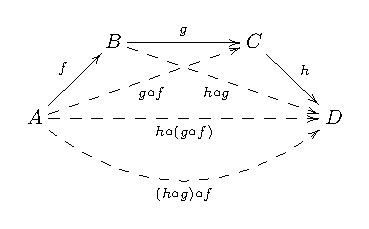
\includegraphics[scale=1.1]{doc/representation_matrix/representation_matrix.pdf}
	%	\label{fig:repr_mat}
	%	\caption{Map diagram of the representation matrix}
\end{figure}
The 'C' means that the diagram is commutative.

Since $\Phi^{-1}_{\mathcal{B}}, T, \Phi_{\mathcal{C}}$ are all linear maps, the map $\Phi_{\mathcal{C}} \circ T \circ \Phi^{-1}_{\mathcal{B}}: K^n \to K^m$ is also linear. By Lemma \ref{lem*mat_unique_lin_map}, any linear map $K^n \to K^m$ can be written using a matrix $A \in M_{m \times n}(K)$. In other words, there exists a unique matrix $A \in M_{m \times n}(K)$ s.t. $\Phi_{\mathcal{C}} \circ T \circ \Phi^{-1}_{\mathcal{B}} = T_A$. The matrix $A$ is called the \textbf{representation matrix of T w.r.t. the bases $\mathcal{B}$ and $\mathcal{C}$}. We denote this matrix by $[T]^{\mathcal{B}}_{\mathcal{C}} \in M_{m \times n}(K)$.

\subsubsection{Entries of the Representation Matrix}
Let $T:V \to W$ be a linear map and $\mathcal{B} = (v_1, \hdots , v_n)$ a basis for $V$, and $\mathcal{C} = (w_1, \hdots , w_m)$ a basis for $W$.
\begin{figure}[H]
	\centering
	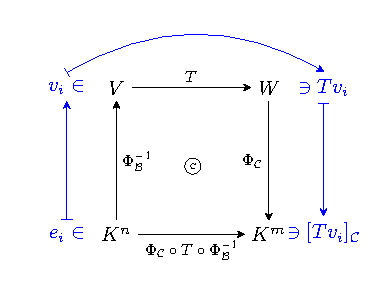
\includegraphics[scale=1.1]{doc/representation_matrix_2/representation_matrix_2.pdf}
\end{figure}
$T_A(e_i) = \Phi_{\mathcal{C}} \circ T \circ \Phi^{-1}_{\mathcal{B}}(e_i) = \Phi_{\mathcal{C}} \circ Tv_i = [Tv_i]_{\mathcal{C}}$. But these are precisely the columns of $A$. In other words
\[
A = [T]^{\mathcal{B}}_{\mathcal{C}} = \begin{pmatrix}
	\rule{0.5pt}{2ex} & & \rule{0.5pt}{2ex}\\
	[Tv_1]_{\mathcal{C}} & \hdots & [Tv_n]_{\mathcal{C}}\\
	\rule{0.5pt}{2ex} & & \rule{0.5pt}{2ex}\\
\end{pmatrix} \in M_{m\times n}.
\]
Another way to describe this matrix is: Let $A = (a_{i,j})$, where $a_{i,j}$ are defined uniquely by
\[
Tv_j = \sum_{i=1}^{m} a_{ij} w_j.
\]

\begin{proposition}{Represenation matrix}{repr_mat}
	Let $T:V \to W$ be a linear map between two finite dimensional vector spaces $V, W$. Let $\mathcal{B}, \mathcal{C}$ be bases for $V, W$ respectively. Then 
	\[
	\forall v \in V : \, [T]^{\mathcal{B}}_{\mathcal{C}} \cdot [v]_{\mathcal{B}} = [Tv]_{\mathcal{C}}.
	\]
\end{proposition}

\subsubsection{Representing Composition of Linear Maps by Matrices}
Let $T:V \to W, S:W \to U$ be linear maps. Let $\mathcal{A} = (v_1, \hdots , v_n)$ be a basis for $V$, $\mathcal{B} = (w_1, \hdots , w_m)$ a basis for $W$ and $\mathcal{C} = (u_1, \hdots , u_p)$ a basis for $U$.

Write $[T]^{\mathcal{A}}_{\mathcal{B}} = (a_{ij}), [S]^{\mathcal{B}}_{\mathcal{C}} = (b_{ij}), [S \circ T]^{\mathcal{A}}_{\mathcal{C}} = (c_{ij})$. By definition we have that
\begin{align}
	\label{eq:comp_mat_a}
	T(v_j) &= \sum_{k=1}^{m} a_{kj} w_k \qquad \forall 1 \leq j \leq n\\
	\label{eq:comp_mat_b}
	T(w_j) &= \sum_{i=1}^{p} b_{ij} u_i \qquad \forall 1 \leq j \leq m\\
	\label{eq:comp_mat_c}
	S \circ T(v_j) &= \sum_{i=1}^{p} c_{ij} u_i \qquad \forall 1 \leq j \leq n
\end{align}
But we can calculate $S \circ T(v_j)$ by using Equations \eqref{eq:comp_mat_a}, \eqref{eq:comp_mat_b}. Then we have
\begin{align*}
	S \circ T(v_j) &= S\big(\sum_{k=1}^{m} a_{kj} w_k\big) = \sum_{k=1}^{m} a_{kj} S(w_j) = \sum_{k=1}^{m} a_{kj} \big(\sum_{i=1}^{p}b_{ik} u_i \big)\\
	&= \sum_{k=1}^{m}\sum_{i=1}^{p} a_{kj}b_{ik} u_i = \sum_{i=1}^{p}\sum_{k=1}^{m} a_{kj}b_{ik} u_i = \sum_{i=1}^{p} \big(\sum_{k=1}^{m} b_{ik}a_{kj}\big) u_i\\
	\Longrightarrow \quad c_{ij} &= \sum_{k=1}^{m} b_{ik}a_{kj}.
\end{align*}
